

\documentclass[DIV=calc, paper=a4, fontsize=13pt, twocolumn]{scrartcl}	 % A4 paper and 11pt font size

\usepackage{lipsum} % Used for inserting dummy 'Lorem ipsum' text into the template
\usepackage[english]{babel} % English language/hyphenation
\usepackage[protrusion=true,expansion=true]{microtype} % Better typography
\usepackage{amsmath,amsfonts,amsthm} % Math packages
\usepackage[svgnames]{xcolor} % Enabling colors by their 'svgnames'
\usepackage[hang, small,labelfont=bf,up,textfont=it,up]{caption} % Custom captions under/above floats in tables or figures
\usepackage{booktabs} % Horizontal rules in tables
\usepackage{fix-cm}	 % Custom font sizes - used for the initial letter in the document

\usepackage{sectsty} % Enables custom section titles
\allsectionsfont{\usefont{OT1}{phv}{b}{n}} % Change the font of all section commands

\usepackage{fancyhdr} % Needed to define custom headers/footers
\pagestyle{fancy} % Enables the custom headers/footers
\usepackage{lastpage} % Used to determine the number of pages in the document (for "Page X of Total")
\usepackage{listings}
\usepackage{graphicx}
%\graphicspath{ {Triplex MDH 140 C} }
 
 


% Headers - all currently empty
\lhead{}
\chead{}
\rhead{}

% Footers
\lfoot{}
\cfoot{}
\rfoot{\footnotesize Page \thepage\ of \pageref{LastPage}} % "Page 1 of 2"

\renewcommand{\headrulewidth}{0.0pt} % No header rule
\renewcommand{\footrulewidth}{0.4pt} % Thin footer rule

\usepackage{lettrine} % Package to accentuate the first letter of the text
\newcommand{\initial}[1]{ % Defines the command and style for the first letter
\lettrine[lines=3,lhang=0.3,nindent=0em]{
\color{DarkGoldenrod}
{\textsf{#1}}}{}}

%----------------------------------------------------------------------------------------
%	TITLE SECTION
%----------------------------------------------------------------------------------------

\usepackage{titling} % Allows custom title configuration

\newcommand{\HorRule}{\color{DarkGoldenrod} \rule{\linewidth}{1pt}} % Defines the gold horizontal rule around the title

\pretitle{\vspace{-30pt} \begin{flushleft} \HorRule \fontsize{50}{50} \usefont{OT1}{phv}{b}{n} \color{DarkRed} \selectfont} % Horizontal rule before the title

\title{Mandatory Project 3} % Your article title

\posttitle{\par\end{flushleft}\vskip 0.5em} % Whitespace under the title

\preauthor{\begin{flushleft}\large \lineskip 0.5em \usefont{OT1}{phv}{b}{sl} \color{DarkRed}} % Author font configuration

\author{Sebastian Gjertsen, } % Your name

\postauthor{\footnotesize \usefont{OT1}{phv}{m}{sl} \color{DarkBlue} % Configuration for the institution name
University of Oslo % Your institution

\par\end{flushleft}\HorRule} % Horizontal rule after the title

\date{} % Add a date here if you would like one to appear underneath the title block

%----------------------------------------------------------------------------------------

\begin{document}

\maketitle % Print the title

\thispagestyle{fancy} % Enabling the custom headers/footers for the first page 

%----------------------------------------------------------------------------------------
%	ABSTRACT
%----------------------------------------------------------------------------------------


%----------------------------------------------------------------------------------------
%	ARTICLE CONTENTS
%----------------------------------------------------------------------------------------


%------------------------------------------------


\section*{1}
\begin{figure}[h]
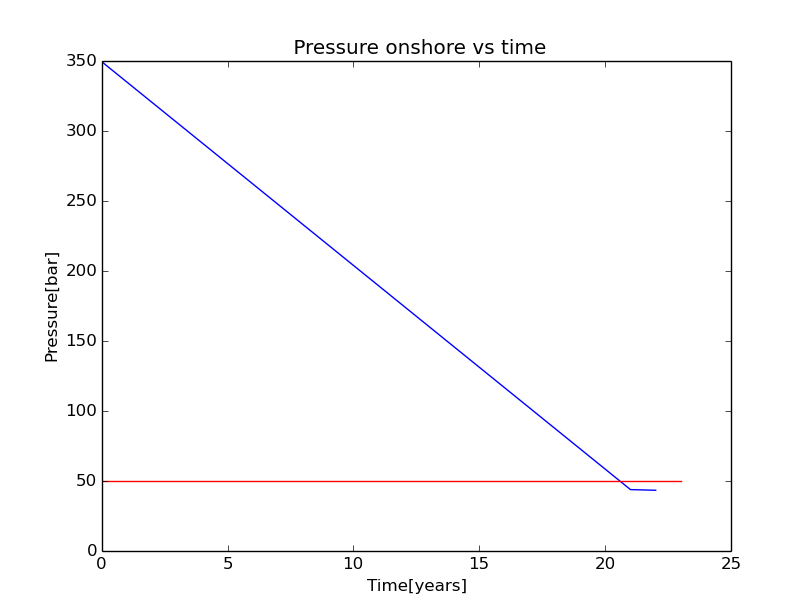
\includegraphics[width=9cm,height=8cm]{Pressure_years.png}
\end{figure}
\subsection*{b)}
As we can see from the plot we will need to install pressure support after about 21 years.
\subsection*{c)}
The liquid is neglected since the GOR is large. So we have mainly gas in our pipe. The main uncertainty with this approximation is that we think of the fluid as incompressible and therefore set the density constant in the well and flowline. We know that gas can be a highly compressible so that the density will change for different pressures and temperatures anywhere in the well or flowline.
\newline
Also the liquid that is in the well will be more dense, and therefore give more pressure drop than only gas.
\subsection*{d)}
To improve the calculations. We could use a different approximation for the friction factor. The Darcy - Weisbach factor has a discontinuity when moving from laminar to turbulent flow. (But we never reach Reynolds numbers under 2300, so it should be okay). 
\subsection*{f)}
If we choose to install a compressor subsea, we will run into these problems:
\begin{itemize}
\item Slugging, a problem of slugging can occur when we have multiphase flow coming from the well. These changes in pressure and force can seriously damage equipment. To tackle this problem we can install a separator which separates the water from the gas and oil. This gives us a simpler flow with less slugging.
\item Droplets, even though we have a separator we can get droplets in the gas. When we use a compressor on a fluid which have droplets(with some incompressible parts) the stress on the equipment can become large, and destroy precious gear. Droplets can also lead to a reduction in the effectiveness of the compressor. This problem can be solved by installing a scrubber before the compressor, which takes out some of the liquid.
\item Deposits, another problem is chemical deposits which are in the flow. Which under compression will in similar fashion to droplets can destroy equipment. We can solve this by adding chemicals in the flow to dissolve these deposits into liquid or gas. This will ease the stress on the equipment
\end{itemize}

\subsection*{g)}
Installing a compressor subsea is a difficult task but will ultimately bring many benefits:
\begin{itemize}
\item Placing the compressor closer to the well will make i more effective. This can give the well a longer life and better production. With a subsea compressor it is also possible to transport the hydrocarbons longer.
\item Installing anything subsea is always a very difficult task. Just getting electricity down many thousands of meters can be a difficult task. Though it will use less electricity than a topside compressor. Maintenance also becomes a problem subsea. It has to be done by an ROV. While maintenance is much easier onshore.
\item Placing compressors on the seabed is a new invention. The Åsgard field by Statoil will be the first to have it. This makes it an unsafe investment, and could have many problems. Making it possibly unreliable.
\end{itemize}
- Electricity to subsea compressor, no problem topside
- More difficult to install subsea, and maintenance 
- Higher and longer production with subsea
- Closer the compressor is to the well, the more effective.
- Subsea compressor is a new invention. May be unreliable

\subsection*{h)}
\begin{figure}[h]
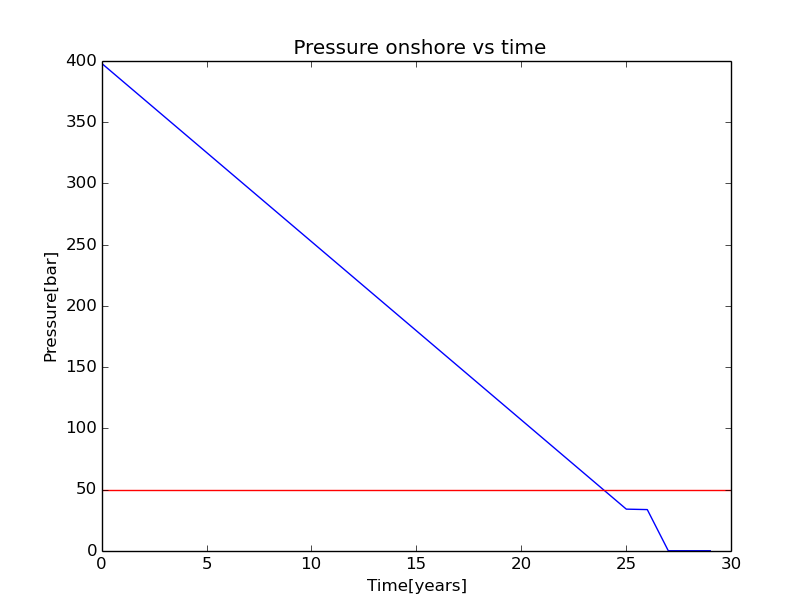
\includegraphics[width=9cm,height=8cm]{Pressure_compressor.png}
\end{figure}
We can see from the figure when we have a compressor with an extra 50 bar from the start we can extend the production by 3-4 years. Installing the compressor from the start will give us more production and it also will not give us any down time if we have to install the compressor at a later stage in the production. 



- Down time while installing compressor, not if installed from start
\newpage
\section*{2}
Issues in the flow will be:
\begin{itemize}
\item Slugs
\item Hydrates
\item Wax
\end{itemize}
In the next sections i will calculate and give ways of tackling these problems
\subsection*{a)}
To calculate the temperature 
I have used equation (57) and not (58) to calculate the temperature drop, since the pressure is constant from reservoir to well and from well to onshore.
In the figures we see the temperatures from the reservoir to the well and from the well to onshore. The different plots are for different mass flow rates from the different years.
\begin{figure}[h]
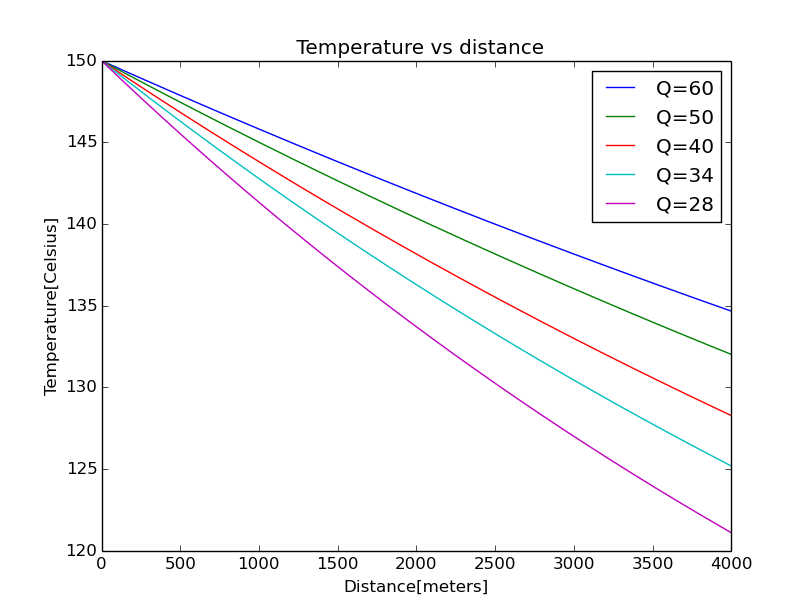
\includegraphics[width=9cm,height=8.5cm]{Temp1.png}
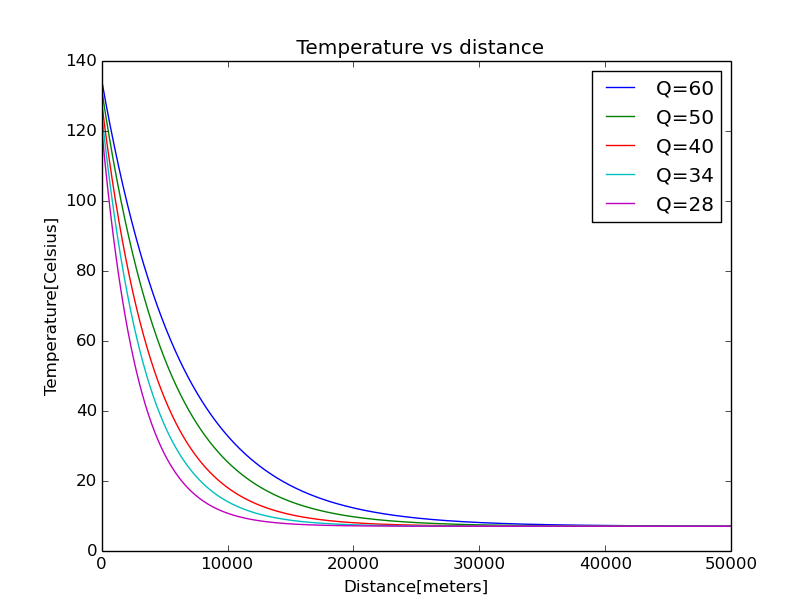
\includegraphics[width=9cm,height=8.5cm]{temp2.png}
\end{figure}
\subsection*{b)}
As we see from the first figure, that we will have high enough temperatures from reservoir to well. But in the second figure, we see that between 1000-2000 m, in the flowline, we hit temperatures low enough so that hydrates will form. 
The hydrates can be dealt with be adding chemicals to the flow, to stop the hydrates from forming. We can add chemicals like methanol(MeOH or MEG). 
\newline
If we have a subsea compressor, this will increase the temperature, and will hopefully prevent hydrates from forming. 
\newline
The hydrates can be prevented from happening if we can avoid low temperatures. This can be done by have sufficiently insulation in the flow line.
\subsection*{c)}
In the flowline we will hit temperatures and pressures under WAT. So that wax will form in the flowline. When wax starts to form and the circumference of the line begins to lessen, giving us less fluid flux and therefore less production. We will need to pig the line. Where we start with a smaller pig and increasing the size, so to get all of the wax out from the line. It is also possible to use steam to remove the wax, though this is an expensive venture.
Since we have a high GOR, the WAT can be manipulated through separation in the line.
\section*{3}
Hydrates form in gas wells that have high pressure and low temperature, where natural gas and water is present
The best way to make sure that we do not have hydrates forming. Is to make sure the temperature of the fluid is above the hydrate forming temperature. If a subsea compressor is installed this will give us higher temperatures, which will help in preventing hydrate formation.
\newline
Having control over the amount of water in the line is also an important factor in hydrate management. If we separate the water from the hydrocarbons and pump it back into the reservoir, this will help in preventing hydrates.
\newline
It is also possible to add chemicals, like salt solution or alcohol, so that we effectively push the hydrate formation domain.

\section*{4}
\begin{figure}[h]
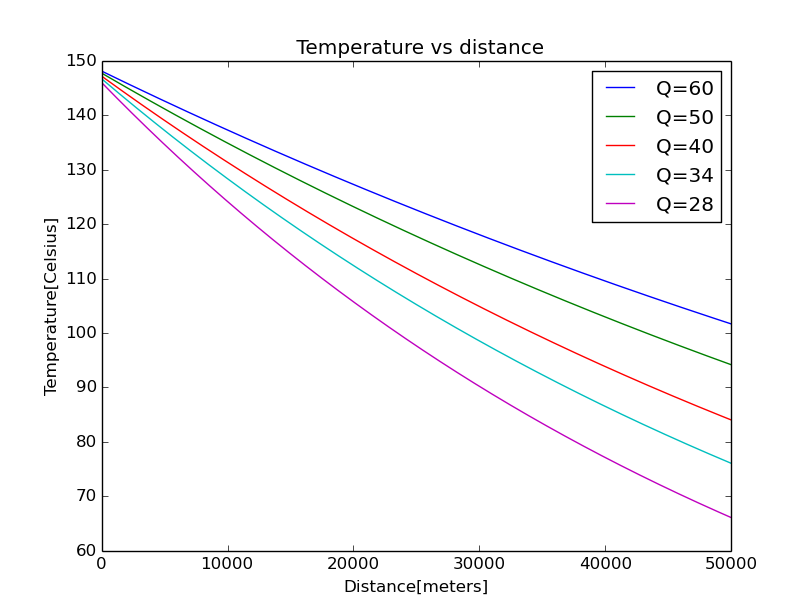
\includegraphics[width=9cm,height=8.5cm]{Temp_insulated.png}
\end{figure}
\subsection*{a)}
We see in the figure that when we lower the heat transfer coefficient, which means that the pipe will be more insulated in some way, that we hold a higher temperature. With higher temperature the fluid will be over the hydrate forming domain, so that hydrates will not form. The same with the wax. With higher temperatures we see from the wax appearance curve that wax will not appear.

\section*{5}
In general vibrations are caused by rapid changes in pressure, which again is caused by changes in density. Since we assume constant density reservoir to well, vibration will not be a huge problem.
\newline
However, if we have inlets in the x-mas tree that we do not use, so called dead-leg. Acoustic pulsations can occur. If these pulsations matches the eigenfrequency of the tubing, then vibrations will occur. Though it can be argued that these effects are not flow induced but rather geometry induced. 
\newline
A common flow inducer are slugs. But with the high GOR in this flow. This will not be a problem. 
\newline
Vibrations may occur at connection spots. And with many connection points and complex routes for the flow to go through. It is very hard to not hit one of the eigenfrequencies. Therefore the best strategy will be to construct the x-mas tree to with stand vibration until after production is over  

\subsection*{a)}
\begin{itemize}
\item First thing to consider when designing a subsea development, is to know what type of hydrocarbons will be produced. 
\item Separation.  We will need to separate out the water and we can inject that water right back into the well to maintain pressure. And to not produce very expensive sea water. Which we cannot sell. This separation is also critical if we send the gas and the liquid to different places. In the case of mainly producing gas in the reservoir, the separation is important if we are to use compression.
\item Compression. Depending on the amount of GOR, the compressor needs to have liquid tolerance matching this ratio. Demanding a multiphase compressor. Depending also on how well we can separate the gas, we can use a compressor with low liquid tolerance. 
\item Cooling. Depending on the temperature of the liquids from the well. The equipment may not tolerate high temperatures and temperature changes. So it may need to be cooled down. By changing the temperature we also change the density of the fluid. And can change the phases of the fluids.
\item Power. All subsea processing needs power. The amount of power needed will be different for each system. Regardless the power lines need to be watertight. 
\item Monitoring. Many parameters in the flow needs to be monitored. Including, pressure, temperature, sand detection and vibration.
\end{itemize}
- Boosting/ Compression , multiphase? Gas or oil, if gas compression, if oil pump? Liquid tolerance
- Separation, putting water right back
- Cooling, how hot is the HC
- Flow assurance
- Power
- Multiphase pump
- Length to tieback
- Monitoring

\section*{6}
A subsea x-mas tree is the device that sits on top of the well head, where the hydrocarbons flow from the reservoir. It is basically used to control the flow coming from the reservoir. I have added a picture of a x-mas tree which is not for subsea, but it clearly shows the properties of a x-mas tree. The subsea x-mas tree has the same functions and some additional functions. The x-mas tree in the yellow color is a subsea x-mas tree. It is not so easy to spot the functions. The main functions are
\begin{itemize}
\item Controls flow from the well, (from picture) in this case with two master valves which can be used to shut the flow completely in case of emergency. These will normally also be hydraulically driven to stay open, so that if something goes wrong, like the power goes out, the valve will automatically close. 
\item The x-mas tree, in this case on the left side(picture), has injection points for chemicals. This is used as we know to help control the buildup of wax and hydrates.
\item The x-mas tree can also have points for injection back into the well, for old wells to prolong production.
\item It has monitoring options to monitor temperature, sand, flow rate, pressure and other things. It can also receive signals from the well and automatically give a response.
\item The x-mas tree can also function as a pressure reliever, if the pressure from the reservoir is to high for the system to handle.
\item The valve on top is used for intervention to the well. Like putting in wireline to lower down equipment, or to take measurements 
\item The subsea x-mas tree has also a vibration monitor. To monitor for instance flow induced vibrations.
\end{itemize}


Main function of a subsea flow tree:
- Control flow of oil and gas out of the well
- Control injection in an old field
- chemical injection
- monitoring(such as pressure, temperature, corrosion, erosion, sand detection, flow rate, flow composition, valve ,choke position feedback)
- pressure relief
- react to sensors from the well 
- Wellhead and tree are not the same, tree is on top of wellhead
- Many valves
- Shutdown of valves(hydraulics maybe) in case of emergency(failsafe needs power to stay open)
\begin{figure}[h]
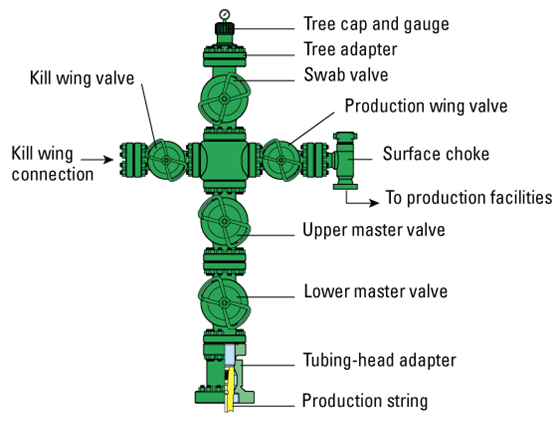
\includegraphics[width=9cm,height=8.5cm]{xmas_tree_diagram.png}
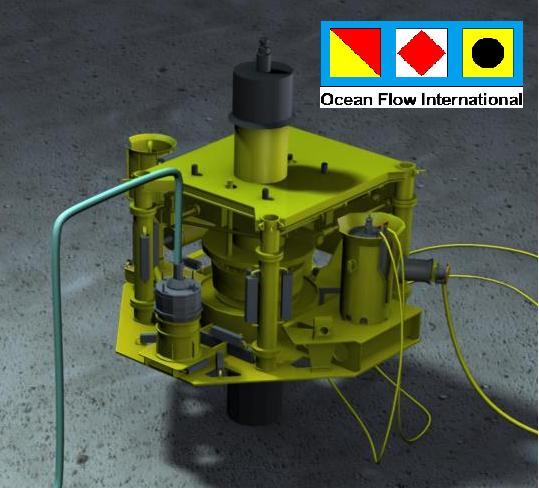
\includegraphics[width=9cm,height=8.5cm]{Ocean_Flow_Subsea_Tree_002.JPG}
\end{figure}




















%----------------------------------------------------------------------------------------
%	REFERENCE LIST
%----------------------------------------------------------------------------------------
\newpage
\begin{thebibliography}{99} % Bibliography - this is intentionally simple in this template


\newblock http://www.croftsystems.net/blog/the-difference-between-a-wellhead-christmas-tree
 
\end{thebibliography}


%----------------------------------------------------------------------------------------

\end{document}